\documentclass[20pt,landscape,pdftex]{foils}

\usepackage{ppftlk}
\usepackage{pause}
\usepackage{background}
\usepackage{mpmulti}
\usepackage{hyperref}
\usepackage{pp4link}

\renewcommand{\P}{\text{P}}
\newcommand{\MC}{\multicolumn}
\renewcommand\r{\right}
\renewcommand\l{\left}
\newcommand\dist{\buildrel\rm d\over\sim}
\newcommand\ind{\stackrel{\rm indep.}{\sim}}
\newcommand{\cY}{{\cal Y}}
\newcommand{\cT}{{\cal T}}
\setlength{\doublerulesep}{\arrayrulewidth}
\newtheorem{assumption}{Assumption}
\newcommand{\indep}{{\bot\negthickspace\negthickspace\bot}} 
\newcommand\spacingset[1]{\renewcommand{\baselinestretch}%
{#1}\small\normalsize}

%
\title{Causal Inference in Political Science Research: Matching as
  Nonparametric Preprocessing for Improving Parametric Causal
  Inference}

\date{October 26, 2004}
\author{  Kosuke Imai\\
  Department of Politics\\ Princeton University \\
  \\ \\
  Joint work with \\
  Daniel E. Ho, Yale Law School\\
  Gary King, Harvard University\\
  Elizabeth A. Stuart, Mathematica Policy Research
\mbox{}\pdfbookmark{TitlePage}{stlab0}}

\parindent=0pt
\begin{document}
\color{black}
\LOGOOFF
%\hypersetup{pdfpagetransition={Split /Dm /H /M /O}}
%\hypersetup{pdfpagetransition={Blinds /Dm /H}}
\hypersetup{pdfpagetransition={Box /M /O}}
%\hypersetup{pdfpagetransition==Dissolve}
\maketitle

%%%%%%%%%%%%%%%%%%%%%%%%%%%%%%%%%%%%%%%%%%%%%%%%%%%%%%%%%%%%%%%%%%%%%%%%%%%%%%%

\foilhead{The Problem: Model Sensitivity in Causal Inference\pause}

\hypersetup{pdfpagetransition=Replace}

\begin{itemize}
\item How most political scientists do empirical analysis:\pause
  \begin{enumerate}
  \item collect the data spending months or years.\pause
  \item finish recording and merging.\pause
  \item sit in front of your computer with nobody to bother you.\pause
  \item run one regression.\pause
  \item run another regression with different control variables.\pause
  \item run another regression with different functional forms.\pause
  \item run another regression with different measures.\pause
  \item run yet another regression with a subset of the data.\pause
  \item end up with 100 or 1000 {\it different} estimates.\pause
  \item put 5 regression results in the paper.\pause 
  \end{enumerate}
\item What's the problem?\pause
  \begin{itemize}
  \item ``correct'' specification is chosen after looking at the
    estimates.\pause  
  \item to readers of an article, it's never clear whether it
    represents a true test of an ex ante hypothesis or merely shows
    it's possible to find such results.\pause
  \end{itemize}

\item Our idea: reduce model dependence without introducing
  bias.\pause
  \begin{itemize}
  \item preprocess the data without looking at the estimates.\pause
  \item run the same parametric model on the preprocessed data.\pause
  \end{itemize} 
\end{itemize}


%%%%%%%%%%%%%%%%%%%%%%%%%%%%%%%%%%%%%%%%%%%%%%%%%%%%%%%%%%%%%%%%%%%%%%%%%%%%%%%

\foilhead{Our Proposed Solution: Preprocessing the Data\pause}

\hypersetup{pdfpagetransition=Replace}

\begin{itemize}
\item Matching, a new statistics literature on causal inference:\pause
  \begin{enumerate}
  \item nonparametric, non-model based methods.\pause
  \item reducing or eliminating functional form and other assumptions.\pause
  \end{enumerate}
  
\item But, from the point of view of practical researchers,\pause
  \begin{enumerate}    
  \item conflicting techniques, practices, guidelines, and rules of
    thumbs.\pause 
  \item calculation of valid standard errors is complicated or
    unavailable.\pause
  \item few theoretical results.\pause
  \end{enumerate}

\item Our unifying idea of this diverse literature:\pause 
  \begin{enumerate}
  \item use matching NOT as a substitute for familiar parametric
    regression analysis.\pause
  \item use matching to make conventional parametric models work
    better.\pause 
  \end{enumerate}

\item Under our proposed framework,\pause
  \begin{enumerate}
  \item parametric analyses are applied to preprocessed data rather
    than to raw data.\pause
  \item valid standard errors are readily available.\pause
  \item resulting estimates are less model dependent.\pause
  \end{enumerate} 

\end{itemize}

%%%%%%%%%%%%%%%%%%%%%%%%%%%%%%%%%%%%%%%%%%%%%%%%%%%%%%%%%%%%%%%%%%%%%%%%%%%%%%%

\foilhead{What is Causal Inference?\pause}

\hypersetup{pdfpagetransition=Replace}

\begin{itemize}
\item We think we are making causal inferences, but what exactly is
  causal inference?\pause
  
\item Causal inference requires counterfactual outcomes as well as
  factual ones.\pause
  \begin{enumerate}
  \item The budget deficit has risen because President Bush
    implemented a tax cut.\pause\\
    The budget deficit would not have risen if he had not
    implemented a tax cut.\pause\\

  \item Reagan was elected president in 1984 because he was an incumbent.\pause\\
    Reagan would not have been elected in 1984 if he were not an
    incumbent.\pause\\ 
    
  \item Hillary Clinton voted for a child care bill because she is a woman.\pause\\
    Hillary Clinton would not have voted for the bill if she were not
    a woman.\pause
  \end{enumerate}  
  
\item Whether qualitatively or quantitatively, you must infer
  counterfactual outcomes (what you don't observe) from factual
  outcomes (what you observe).\pause

\item Some causal inference is more difficult than others.\pause
      
\item Causal inference requires assumptions and yields uncertainty.\pause

\item Causality is different from association.\pause

\end{itemize}


%%%%%%%%%%%%%%%%%%%%%%%%%%%%%%%%%%%%%%%%%%%%%%%%%%%%%%%%%%%%%%%%%%%%%%%%%%%%%%%

\foilhead{Formal Definition of Causal Effects\pause}

\hypersetup{pdfpagetransition=Replace}

\begin{itemize}

\item Notations:\pause
  \begin{itemize}
  \item Units:  $i=1,\dots,n$.\pause
  \item Observed treatment: $t_i=1$ if treated, $t_i=0$ otherwise.\pause
  \item Observed outcome: $y_i$.\pause
  \item Control variables: {\it pre}treatment variables $X_i$.\pause
  \end{itemize}
  
\item Potential outcomes framework (Rubin Causal Model): 
  \begin{itemize}
  \item $y_i(1) \equiv y_i(t_i=1)$ and $y_i(0) \equiv y_i(t_i=0)$.\pause  \\
    
    \begin{tabular}{ccc}
      Units & $y_i(1)$ & $y_i(0)$ \\
      \hline
      1 & 15  & ? \\
      2 &  ?  & 10 \\ 
      3 &  ?  & 8 \\
      \vdots & \vdots & \vdots \\
      $n$ & 20 & ? \\
      \hline
    \end{tabular} \pause \\ \\
    
  \item Realized Causal Effect for unit $i$: $y_i(1) - y_i(0)$.\pause
  \item The fundamental problem of causal inference: $y_i = t_i y_i(1) +
    (1-t_i)y_i(0)$.\pause
  \item Random causal effect for unit $i$: $Y_i(1) - Y_i(0).$\pause
  \item Mean causal effect for unit $i$: $E[Y_i(1) - Y_i(0)].$\pause
  \end{itemize}

%%%%%%%%%%%%%%%%%%%%%%%%%%%%%%%%%%%%%%%%%%%%%%%%%%%%%%%%%%%%%%%%%%%%%%%%%%%%%%%

\foilhead{Basic Assumptions and Quantities of Interest\pause}

\hypersetup{pdfpagetransition=Replace}

\item Assumptions:\pause
  \begin{enumerate}
  \item No omitted variable bias: $Y_i(t_i) \perp T_i \mid X_i$ for
    all $i$ and $t_i$.\pause
  \item No posttreatment bias: $X_i$ is causally prior to $T_i$.\pause
  \item No interference among units: $Y_i(t_i) \perp T_j$ for all $j
    \ne i$.\pause
  \item Same version of treatment.\pause
  \end{enumerate}

\item Quantities of interest:\pause
  \begin{itemize}
    \item Average Treatment Effect: $ATE = \frac{1}{n}\sum_{i=1}^n
      E[Y_i(1) - Y_i(0)].$\pause 
      \bigskip
    \item ATT for the Treated: $ATT = \frac{1}{\sum_{i=1}^n
        t_i}\sum_{i:t_i=1} E[Y_i(1) - Y_i(0)].$\pause
  \end{itemize}

\item Recent Methodological Developments:\pause
  \begin{itemize}
  \item General treatment regimes: Imai \& van Dyk (2004, {\small \it J. of
      the Amer. Stat. Assoc.})\pause
  \item Interference among units: spatial modeling of the dependence
    among units.\pause 
  \end{itemize}

\item How difficult is causal inference?\pause
  \begin{itemize}
  \item Severe missing data problem: must impute one potential outcome for
    each unit.\pause
  \item As challenging as ecological inference: $y_i = t_i y_i(1) +
    (1-t_i) y_i(0)$ where $y_i$ (observed) is overall turnout,
    $y_i(1)$ is black turnout, $y_i(0)$ is white turnout, and $t_i$
    (observed) is proportion of black voters.\pause
  \end{itemize}

\end{itemize}

%%%%%%%%%%%%%%%%%%%%%%%%%%%%%%%%%%%%%%%%%%%%%%%%%%%%%%%%%%%%%%%%%%%%%%%%%%%%%%%

\foilhead{Data Collection Mechanisms\pause}

\hypersetup{pdfpagetransition=Replace}

\begin{itemize}
\item Classical randomized experiments ($\approx$ 0\% of political
  science research):\pause
  \begin{enumerate}
  \item random selection of units from a given population.\pause
  \item random assignment of values of the treatment.\pause
  \item large $n$.\pause
  \end{enumerate}

\item Other types of randomized experiments ($\approx$ 1\% of
  political science research):\pause

  \begin{itemize}
  \item Natural experiments:  Vietnam draft lottery, California alphabet lottery.\pause
  \item Laboratory, Survey, and Field experiments.\pause
  \item Methodological challenges: sample selection, noncompliance,
    missing data, interference among units.\pause
  \end{itemize}
  
\item Observational studies ($\approx$ 99\% of political science
  research):\pause
  \begin{itemize}
  \item Do not meet the three standards of classical randomized
    experiments.\pause
  \item Comprise almost all political science research.\pause
  \end{itemize}

\end{itemize}



%%%%%%%%%%%%%%%%%%%%%%%%%%%%%%%%%%%%%%%%%%%%%%%%%%%%%%%%%%%%%%%%%%%%%%%%%%%%%%%

\foilhead{Parametric Analysis Methods\pause}

\hypersetup{pdfpagetransition=Replace}

\begin{itemize}
\item Researchers typically assume a parametric model (up to unknown
  parameters):\\ e.g., $Y_i \sim p(\mu_i, \theta)$ with $\mu_i \equiv
  E(Y_i \mid t_i, X_i)=g(\alpha+t_i \beta + X_i \gamma)$\pause
  \begin{itemize}
  \item includes linear regression, logit, probit, poisson, etc.\pause 
  \end{itemize}
  
\item But, in both experimental and observational studies, the true
  model is unknown.\pause

\item In experimental studies, $T_i$ and $X_i$ are independent.\pause
  \begin{itemize}
  \item So $X_i$ can be ignored: $ATT = g(\alpha+\beta) - g(\alpha).$\pause
  \item Then, the results do not depend on the functional form,
    $g(\cdot)$.\pause
  \item Controlling $X_i$ improves the efficiency, but increases
    model dependence.\pause
  \end{itemize}
  
\item In observational studies, the results are {\it always}
  model-dependent:\pause
\begin{itemize}
  \item The main problem: curse of dimensionality\pause
    \begin{itemize}
    \item one 10-category variable requires $10$ parameters (NOT one)
      in regression.\pause
    \item two 10-category variables require $100$ parameters (NOT two).\pause
    \item eight 10-category variables require more parameters than the
      estimated number of elementary particles in the universe.\pause
    \end{itemize}
  \item Other problems: non-normal data, etc.\pause
  \end{itemize}
\end{itemize}

%%%%%%%%%%%%%%%%%%%%%%%%%%%%%%%%%%%%%%%%%%%%%%%%%%%%%%%%%%%%%%%%%%%%%%%%%%%%%%%

\foilhead{Matching as Nonparametric Preprocessing\pause}

\hypersetup{pdfpagetransition=Replace}

\begin{itemize}
\item The Idea: Adjust the data {\it prior to} the parametric analysis
  so that the relationship between $t_i$ and $X_i$ is eliminated or
  reduced.\pause
  
\item Fundamental rule for avoiding selection bias: do not select on
  dependent variable.\pause
  \begin{itemize}
  \item valid selection rule -- a function of $t_i$ and $X_i$.\pause 
  \item randomized blocks in experiments, stratified sampling in
    surveys.\pause
  \end{itemize}

\item Matching methods find a pair (or a group) of control and treated
  units that are ``similar'' to each other in terms of their control
  variables, $X_i$.

\item Preprocessed data set contains a subset of the raw data where
  all units share identical or similar underlying characteristics.\pause

\item Use the same parametric model to analyze the preprocessed data
  set.\pause 
  \begin{itemize}
  \item Model-dependence is reduced because $t_i$ no longer depends on
    $X_i$.\pause
  \item $p(X \mid t=1) = p(X \mid t=0)$ or $p(X \mid t=1) \approx
    p(X\mid t=0)$.\pause
  \item Remaining dependence between $t_i$ and $X_i$, if any, can be
    adjusted by the parametric analysis.\pause
  \end{itemize}
  

\end{itemize}

%%%%%%%%%%%%%%%%%%%%%%%%%%%%%%%%%%%%%%%%%%%%%%%%%%%%%%%%%%%%%%%%%%%%%%%%%%%%%%%

\foilhead{Illustration of How Matching Reduces Model Dependence\pause}

\hypersetup{pdfpagetransition=Replace}

\begin{itemize}
\item An artificial data set with one control variable.\pause
\item Fit two regressions (with/without a quadratic term) before and
  after matching.\pause
\end{itemize}

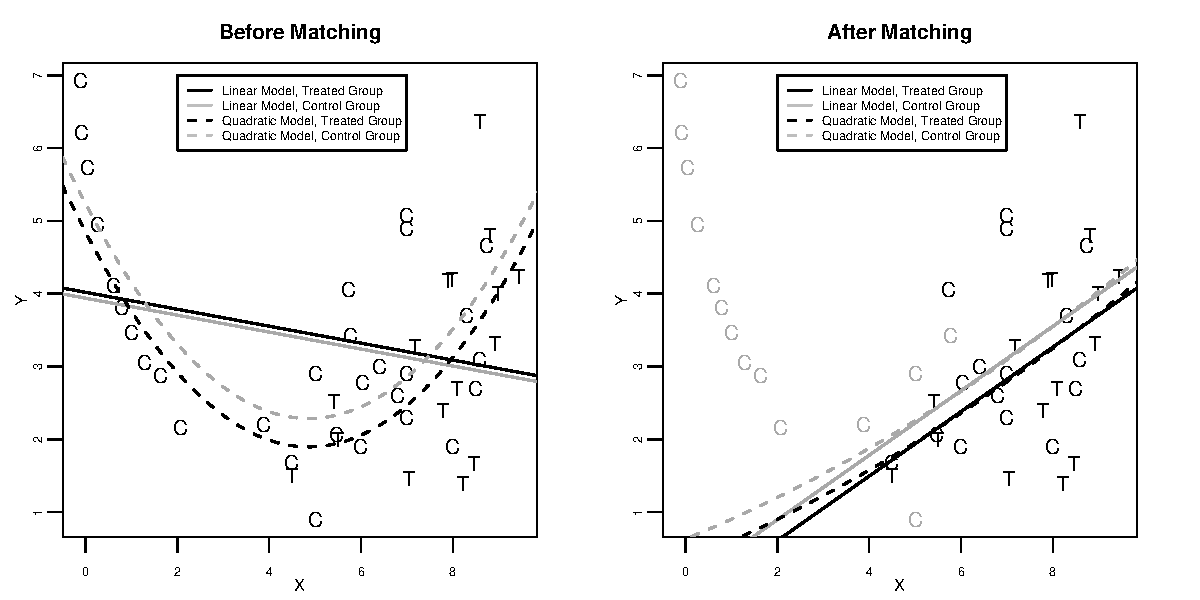
\includegraphics[scale=1.35]{olspanel-thick.pdf}\pause

%%%%%%%%%%%%%%%%%%%%%%%%%%%%%%%%%%%%%%%%%%%%%%%%%%%%%%%%%%%%%%%%%%%%%%%%%%%%%%%

\foilhead{Choosing a Matching Procedure\pause}

\hypersetup{pdfpagetransition=Replace}

\begin{itemize}
\item The goal of matching: improve balance without losing too many
  observations.\pause

\item Try different matching procedures until better balance is
  achieved.\pause

\item But, do not examine the outcome variable during
  preprocessing.\pause

\end{itemize}

\noindent {\bf Step 1:} Select covariates: include at least all the
variables that would have been included in the parametric model, but
avoid posttreatment bias.\pause
  
\noindent {\bf Step 2:} Try exact matching: if a large number of units
are matched, go to the parametric analysis.\pause
  
\noindent {\bf Step 3:} Try various propensity score matching methods:
propensity score summarizes all the variables in $X$ with a single
variable.\pause
  
\noindent {\bf Step 4:} Evaluate the matching procedure: look at various
low-dimensional summaries of $X$.\pause
  
\noindent {\bf Step 5:} Parametric outcome analysis: same method, same
algorithm, same software, same model checking procedures, ...\pause

%%%%%%%%%%%%%%%%%%%%%%%%%%%%%%%%%%%%%%%%%%%%%%%%%%%%%%%%%%%%%%%%%%%%%%%%%%%%%%%

\foilhead{Propensity Score Methods\pause}

\hypersetup{pdfpagetransition=Replace}

\begin{itemize}
\item Defined as the probability of receiving the treatment: 
 $e(X_i)=\Pr(T_i=1\mid X_i)$.\pause
  
\item Rosenbaum and Rubin (1984) proved the key properties:\pause
  \begin{enumerate}
  \item balancing score: $\Pr(T = 1 \mid e(X), X) = \Pr(T = 1
    \mid e(X))$.\pause 
  \item univariate summary of $X$: $Y(t) \perp T \mid e(X)$
    for all $t$.\pause
  \end{enumerate}

\item Matching on propensity score is much easier than matching on $X$.\pause 

\item Propensity score tautology: it works when it works, and when
  it doesn't work, it doesn't work (or keep trying at it).\pause
  
  \begin{itemize}
  \item In observational studies, the true propensity score is
    unknown.\pause
  \item Same model-dependence problem applies to estimation of
    propensity score!\pause
  \item If propensity score is correctly estimated, it should balance
    the covariates.\pause
  \item If balance is not achieved, go back and reestimate propensity
    score.\pause
  \item Use logistic regression, GAM, CART, neural network, or whatever!\pause
  \end{itemize}

\item Propensity score is a tool to do matching, and the balance
  diagnostics are essential.\pause


\end{itemize}

%%%%%%%%%%%%%%%%%%%%%%%%%%%%%%%%%%%%%%%%%%%%%%%%%%%%%%%%%%%%%%%%%%%%%%%%%%%%%%%

\foilhead{Empirical Illustration: FDA Approval and Liberal Senate\pause}

\hypersetup{pdfpagetransition=Replace}

\begin{itemize}
\item Democratic senate majorities and FDA drug approval time
  (Carpenter 2002).\pause
  \begin{itemize}
  \item Hypothesis: ``expected approval times are greater when
    Democrats control the White House, when the agency's oversight
    committees are more liberal, and when the House and Senate are
    more liberal'' (p.495).\pause
  \item liberal FDA oversight should lead to slower approval of new
    drugs.\pause 
  \end{itemize}

\item Original analysis:\pause
  \begin{itemize}
  \item 408 new drugs (262 approved, 146 pending).\pause
  \item lognormal survival model.\pause
  \item seven oversight variables (median adjusted ADA scores for
    House and Senate Committees as well as for House and Senate
    floors, Democratic Majority in House and Senate, and Democratic
    Presidency).\pause
  \item 18 control variables (clinical factors, firm characteristics,
    media variables, etc.)\pause
  \end{itemize}

\item Our analysis:\pause
  \begin{itemize}
  \item focuses on the causal effect of a Democratic majority in the
    Senate.\pause
  \item omits variables that are highly likely to be affected by the
    treatment.\pause
  \item uses one-to-one propensity score matching.\pause
  \item discards 49 units (2 treated and 17 control units).\pause
  \item runs 262,143 possible specifications and calculates average
    treatment effect.\pause
  \end{itemize}
\end{itemize}

%%%%%%%%%%%%%%%%%%%%%%%%%%%%%%%%%%%%%%%%%%%%%%%%%%%%%%%%%%%%%%%%%%%%%%%%%%%%%%%

\foilhead{Improved Balance... \pause}

\hypersetup{pdfpagetransition=Replace}

\vspace*{1in}
\begin{center}
  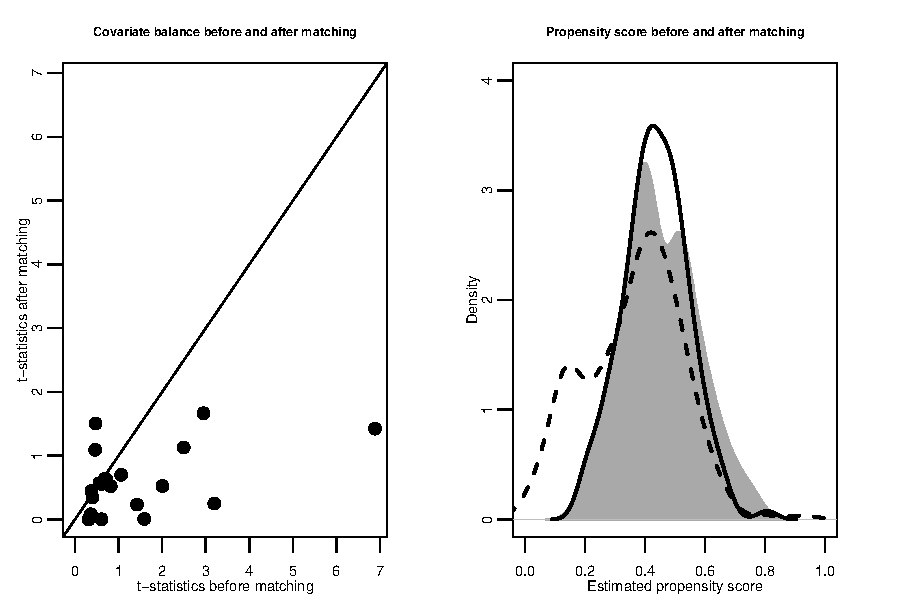
\includegraphics[scale=1.5]{fdabal}\pause 
\end{center}

\foilhead{and Reduced Model Dependence\pause}

\hypersetup{pdfpagetransition=Replace}

\vspace*{1in}
\begin{center}
  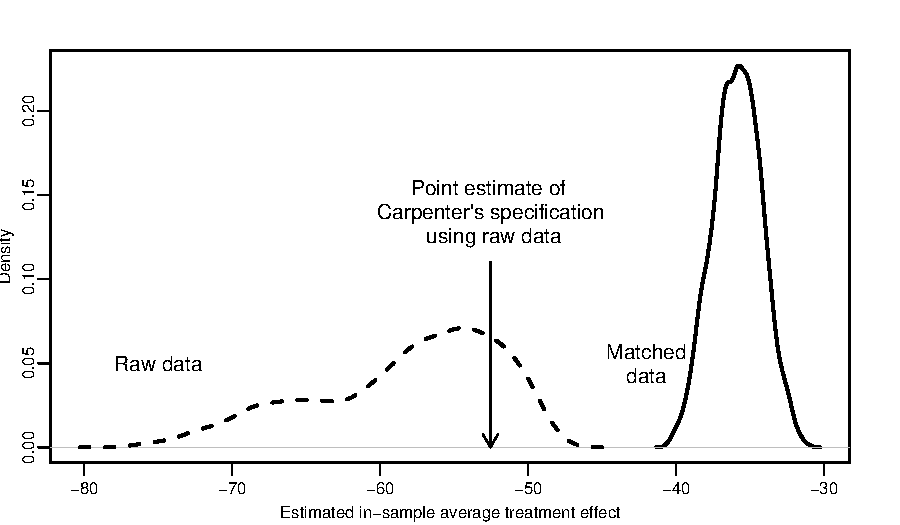
\includegraphics[scale=1.5]{fdadens}\pause 
\end{center}

%%%%%%%%%%%%%%%%%%%%%%%%%%%%%%%%%%%%%%%%%%%%%%%%%%%%%%%%%%%%%%%%%%%%%%%%%%%%%%%

\foilhead{Concluding Remarks\pause}

\hypersetup{pdfpagetransition=Replace}

\begin{itemize}

\item What can go wrong\pause
  \begin{itemize}
  \item curse of dimensionality in balance diagnostics.\pause
  \item preprocessing data may increase variance while reducing
    bias.\pause 
  \item change in quantities of interest.\pause
  \end{itemize}
  
\item Causal inference is inherently model-dependent in observational
  studies.\pause

\item We provide a way to get around the ethical and methodological
  problem of choosing a model specification.\pause

\item Preprocessing the raw data with matching procedures makes
  familiar parametric models a more reliable tool.\pause

\item Readers (and authors) need not worry that slightly different
  specifications alter the empirical conclusions.\pause

\item Easy-to-use software: MatchIt available at
  \Ia{http://gking.harvard.edu/matchit/}\pause

\end{itemize}

%%%%%%%%%%%%%%%%%%%%%%%%%%%%%%%%%%%%%%%%%%%%%%%%%%%%%%%%%%%%%%%%%%%%%%%%%%%%%%%

\foilhead{Empirical Illustration: Visibility and Candidate Evaluation\pause}

\hypersetup{pdfpagetransition=Replace}

\begin{itemize}
\item Causal effect of visibility on candidate evaluations (Koch
  2002).\pause
  \begin{itemize}
  \item A candidate is ``visible'' if their campaign expenditure exceeds
    \$750,000.\pause
  \item 494 candidates of US House in the data set.\pause
  \item Pretreatment covariates: candidate ideology, voter perception
    of party ideology, respondent ideology, candidate feeling
    thermometer, and political awareness.\pause
  \item The original analysis used linear regression.\pause
  \end{itemize}

\item Our analysis:
  \begin{itemize}
  \item We ignore possible measurement error, posttreatment bias, and
    interference among units, and focuse on the issue of
    model-sensitivity.\pause
    
  \item The same parametric model with no functional form assumption
    would require 87,530,856 parameters.\pause  
    
  \item We subclassify rather than match on the estimated propensity
    score.\pause
    
  \item Drop 31 observations that fall outside of the common
    support.\pause
  \item Within each subclass, we fit the same parametric model and
    then compute the overall treatment effect as the weighted average
    of within-subclass estimates.\pause
    
  \item Fit 64 possible linear regressions, and examine
    model-sensitivity of the average treatment effect for the treated.\pause
  \end{itemize}
\end{itemize}

%%%%%%%%%%%%%%%%%%%%%%%%%%%%%%%%%%%%%%%%%%%%%%%%%%%%%%%%%%%%%%%%%%%%%%%%%%%%%%%

\foilhead{Improved Balance and Reduced Model Dependence\pause}

\hypersetup{pdfpagetransition=Replace}

\begin{center}
    \begin{tabular}{lrrrrrrr}
      \hline
      & Raw  &\MC{6}{c}{ Subclasses} \\
      Covariate & Data  & 1 &  2 &  3 &  4 &  5 &  6 \\
      \hline
      Candidate Ideology & 12.18 & 2.16 & -0.85 & 0.33 & 1.15 & 1.51 & -0.45 \\
      Party Ideology & -0.42 & -0.65 & -1.05 & 0.59 & 0.24 & 0.06 & 1.53 \\
      Respondent Ideology & -0.97 & 1.45 & -0.73 & 1.08 & -0.38 & -1.26 & -1.00 \\
      Respondent Ideology $\times$ & -0.44 & 0.50 & -0.81 & 1.64 & 0.18 &
      -1.44 & -0.42 \\
      \hspace{0.1in} Feeling Thermometer \\
      Feeling Thermometer & 1.70 & -0.03 & 0.33 & 1.61 & 0.03 & -1.34 & 1.08 \\
      Political Awareness & 2.42 & 0.53 & 0.14 & -1.50 & 0.28 & -1.08 & 0.66
      \\ \hline
      Treated $n$& & 14 & 13 & 13 & 14 & 13 & 11 \\
      Control $n$& & 299 & 30 & 39 & 12 & 3 & 2 \\
      \hline
    \end{tabular} \\
  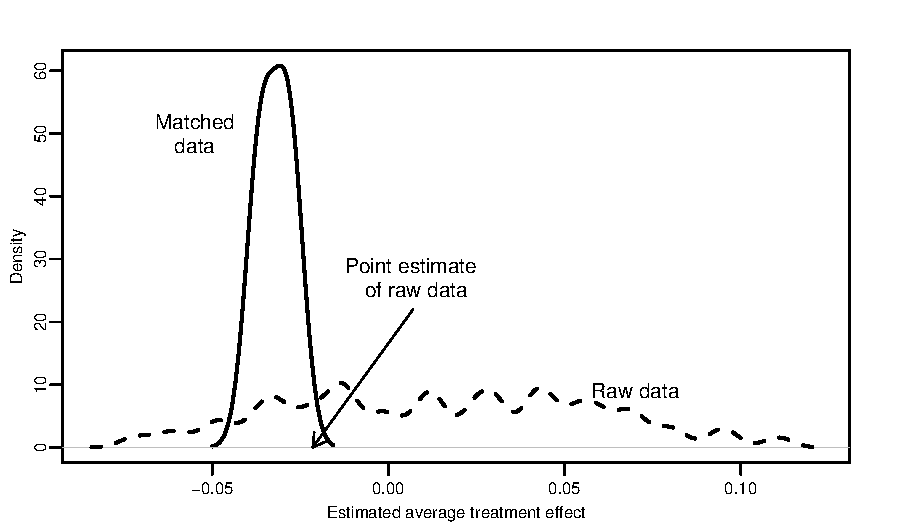
\includegraphics[scale=1]{kochdens}\pause
\end{center}

\end{document}
